% ---------------------------------------------------------------------------
% Problem Set 3: Replication Report Empirical Methods
% The grey instructions are produced by \instr{...}. To hide all of them at once (e.g. to check the length of your report), change \showinstrtrue to \showinstrfalse below. Please remove them before you submit.
% ---------------------------------------------------------------------------
\documentclass[12pt,a4paper]{article}

\usepackage[utf8]{inputenc}
\usepackage[T1]{fontenc}
\usepackage{mathptmx}
\usepackage{microtype}
\usepackage[margin=2.5cm]{geometry}
\usepackage{amsmath,amssymb}
\usepackage{graphicx}
\usepackage{float}
\usepackage{booktabs}
\usepackage{tabularx}
\usepackage{array}
\usepackage{colortbl}
\usepackage{enumitem}
\usepackage{xcolor}
\usepackage[font=small,labelfont=bf,skip=6pt]{caption}
\usepackage[hidelinks]{hyperref}

\setlength{\parindent}{0pt}
\setlength{\parskip}{6pt}
\usepackage{tabularx}
\usepackage{array}
\usepackage{booktabs}
\newcolumntype{L}{>{\raggedright\arraybackslash}X}

% --- Instructions ----------------------------------------------------------
\newif\ifshowinstr
\showinstrtrue
%\showinstrfalse
\newcommand{\instr}[1]{\ifshowinstr{\leavevmode\color{gray}\itshape\small [#1]\par}\fi}

% --- Helpers for the worksheets --------------------------------------------
\newcolumntype{L}{>{\raggedright\arraybackslash}X}
\newcolumntype{P}[1]{>{\raggedright\arraybackslash}p{#1}}
\newcommand{\fillrow}{\rule[-0.35cm]{0pt}{0.85cm}}  % leaves room to write in a row
\newcommand{\rowline}{\arrayrulecolor{black!25}\hline\arrayrulecolor{black}}
\renewcommand{\arraystretch}{1.25}

% --- Table notes -----------------------------------------------------------
\newcommand{\tablenotes}[1]{\par\vspace{4pt}{\footnotesize\textit{Notes:} #1\par}}

\title{Replication of Alesina, Giuliano \& Nunn (2013):\\{} On the Origins of Gender Roles: Women and the Plough}
\author{\begin{tabular}{c@{\hspace{2.5em}}c}Ginevra Bettata & Isimbi Elsa Usanase\\ Leandra Shana Grossniklaus & Rahel Tiffany Gutzwiller\end{tabular}}

\begin{document}
\maketitle

\instr{The grey italic passages provide you with some short instructions. Please delete these passages before you submit by setting \texttt{\textbackslash showinstrfalse} in the preamble. \textbf{The report should be 5 to 7 pages long.} This includes tables and figures but excludes any references and Appendix A. \textbf{Appendix A} tries to guide you through some of the replication exercises. It \textbf{has to be filled in and submitted together with the report}. Appendix~B is only meant as a help for you, and you can delete it before submitting.}

% ===========================================================================
\section{Introduction}
% ===========================================================================
% Problem
Gender norms differ strongly across countries, even among countries with similar income levels. In 2000, female labour force participation was 16.1\% in Pakistan but 90.5\% in Burundi, and the share of people who agree that men should have priority when jobs are scarce ranged from 3.6\% in Iceland to 99.6\% in Egypt. Alesina, Giuliano and Nunn (2013) ask where these differences come from.
% Research question
They test a hypothesis by Ester Boserup (1970): today's gender norms go back to traditional plough agriculture. Unlike the hoe, the plough requires considerable upper-body strength and is difficult to combine with childcare, so men worked in the fields while women specialised in work within the home. This division of labour turned into a belief about women's appropriate role that persisted even after agriculture lost its importance.
% Method and findings
The authors link ethnographic data on which ethnic groups traditionally used the plough to today's countries through the distribution of languages. They relate the share of the population with plough-using ancestors to female labour force participation, female firm ownership and women's political participation, using OLS with historical and contemporary controls. To address the endogeneity of plough adoption, they also estimate 2SLS regressions with the suitability of ancestral land for crops that benefit more or less from the plough as instruments. A country whose population descends entirely from plough-using societies has, on average, 12.9 percentage points lower female labour force participation than a country with no plough tradition (Table IV, column 2); under 2SLS, the difference rises to 25.0 percentage points. Children of immigrants with a plough heritage also work less and hold less equal gender attitudes, which points to cultural persistence as the channel.
% Our contribution
We replicate the OLS and IV results for female labour force participation (Tables III, IV and VIII) exactly. In our extension, we ask whether communist regimes, which actively pushed women into paid work, weakened the plough effect. We find no evidence of this: the implied plough effect is about $-11$ percentage points in (former) communist countries and $-14.5$ in all other countries, and the difference is not significant. Interacting plough use with income gives mostly insignificant results as well. In our critical evaluation, we argue that the main biases in the OLS estimate pull in opposite directions and that the exclusion restriction of the IV is questionable, so the sign of the effect is more credible than its size.

% ===========================================================================
\section{Data and Methodology}
% ===========================================================================

\subsection{Empirical strategy}

\instr{Think about what you need to explain the identification strategy of the authors and why they believe that it is valid. Appendix~B.1 summarizes the main points for OLS, panel data and IV designs. You can use these as a reference.}

The main result comes from a cross-country regression:
\begin{equation}\label{eq:ols}
  FLFP_c = \alpha + \beta\, Plough_c + (X_c^{H})'\gamma + (X_c^{C})'\delta + \mu_{continent} + \varepsilon_c
\end{equation}
$FLFP_c$ is the female labour force participation rate in 2000, expressed as a percentage. $Plough_c$ is the share of the population whose ancestors used the plough, ranging from zero to 1. $X_c^{H}$ contains historical controls describing the ancestors: the agricultural suitability of the land, the tropical climate, the presence of large domesticated animals and the political and economic complexity of the ancestors. The contemporary controls $X_c^{C}$ are the logarithm of real per capita GDP and its square. The term $\mu_{continent}$ captures continent fixed effects.

The authors acknowledge that, however complicated it may be, $\beta$ measures a causal effect only if one assumes that, holding controls constant, plough is not correlated with anything else that might influence female labour force participation. If societies with less egalitarian norms were more likely to adopt the plough, OLS exaggerates the effect. But the plough was also adopted by more developed societies, which today are wealthier and more open to women's labour, and this pushes the estimate toward 0. The authors add a range of other controls (Table VII), but these cannot account for what is not observed.

To identify this effect, the authors turn to two-stage least squares (2SLS). The idea comes from Pryor (1985) who argued that the plough is particularly advantageous for crops that require a large amount of land to be prepared in a short time, on deep and flat soils. The first measure is the suitability of ancestral lands for wheat, barley and rye, for which the plough is highly advantageous (plough-positive environment). The second is the suitability for sorghum and millet, for which the use of the plough was less advantageous (plough-negative environment). The two measures use FAO-GAEZ data on lands within 200 kilometres of the center of each ethnic group, they are divided by the total arable area and aggregated by country using the same population weights as those used for $Plough_c$. We express the first-stage specification described by Alesina, Giuliano and Nunn (2013, p.~516) as follows:
\begin{equation}\label{eq:firststage}
  Plough_c = \pi_0 + \pi_1\, PosEnv_c + \pi_2\, NegEnv_c + X_c'\lambda + \mu_{continent} + u_c
\end{equation}
In the second stage they substitute $Plough_c$ with the value predicted in the first stage in the original regression equation.

The method is based on four assumptions. The first is relevance, whereby, holding controls constant, the instruments must explain plough use. In the first stage (Table VIII, Panel A, Column 2), the coefficient for ``plough-positive'' environment is 0.63 and is highly statistically significant, while that for the ``plough-negative'' environment is not, and the joint F-statistic is 25.06. The second is exogeneity: the instruments must not be correlated with unobserved factors. The authors argue that this is plausible because climate and soil are determined by nature. The third assumption is the exclusion restriction: the types of cereal crops that can be grown must affect current female labour force participation only through plough use. The authors themselves acknowledge that this cannot be taken for granted. The fourth is monotonicity, which is necessary when effects differ across societies and the 2SLS estimates a local effect (LATE). Under this assumption, greater suitability for wheat must never make a society less likely to adopt the plough.

The first threat to this strategy is weak instruments, if the instruments only weakly predict plough use (weak first stage), the 2SLS model approaches OLS and standard tests are unreliable.

The second threat is that the exclusion may not hold. Geography may have shaped development, population density, the emergence of states or nutrition, which in turn may have influenced gender norms. The authors point out that sorghum and millet are often considered inferior grains. In Table A14, they also control for slope, soil depth, temperature and precipitation, but other channels remain possible.

For female labour force participation, the Hansen J test yields a p-value of 0.00 (Table VIII, Panel C, column 2) and thus rejects the hypothesis that both instruments are valid. The test does not indicate which of the two is the problem, and if both violated the exclusion in the same way, it might not detect it.

Another potential threat is measurement error. The plough-use variable is constructed by manually matching 7'612 languages to 1'265 ethnic groups and there is a significant lack of data for Latin America. Classical measurement error in plough use biases the OLS estimate toward zero (attenuation bias), while the 2SLS corrects for it, provided the measurement error is not related to the instruments. This, together with the selection of the most developed countries, could help explain why the IV estimate ($-25.01$) is roughly double that of OLS ($-12.93$). Today's GDP per capita is also likely a consequence of plough and including it among the controls may distort the estimates, however, the authors show that without it, the results change little.

% ===========================================================================
\section{Main Result}
% ===========================================================================

In this section, we replicate the main results of the paper. We first present the OLS estimates and then turn to the IV estimates.

\subsection{Replication}

\instr{This part should include your main replication table (Table~\ref{tab:main}) and figure(s) (at least Figure~\ref{fig:main}). Replicate at least what you consider the main column of the main results table, as well as one or two figures that visualize the result. Do your results differ? Worksheet~A.3 helps you think about why they might differ. It is fine if you cannot replicate a number exactly, as long as you understand why.}

We first replicate the authors' OLS estimates of the relationship between traditional plough use and female labour force participation in 2000. Because plough use is measured as the share of each country's population with plough-using ancestors, the analysis is a cross-country regression with one observation per country. Our main specification estimates equation~\eqref{eq:ols} on 165 countries. Besides plough use, it includes the historical controls, which describe how the ancestors lived, and income, which captures today's level of development. The continent fixed effects mean that each country is only compared with countries on the same continent, so broad regional differences, for example between Africa and Europe, cannot drive the result. As in the paper, standard errors are robust to heteroskedasticity. Table~\ref{tab:main} presents the estimated regressions side by side. Columns (1) and (2) replicate Table III in the paper, which does not yet include income as a contemporary control. Columns (3) and (4) replicate Table IV in the paper, which adds income. Columns (2) and (4) include continent fixed effects, and column (4), which corresponds to Table IV, column (2) in the paper, is our main specification.

\begin{table}[H]
  \centering
  \vspace{-4pt}
  \caption{Country-level OLS estimates of female labour force participation in 2000 (replication of Tables III and IV)}
  \label{tab:main}
  \small
  \renewcommand{\arraystretch}{1}
  \setlength{\tabcolsep}{11.5pt}
  
\begin{tabular}[t]{lcccc}
\toprule
\multicolumn{1}{c}{ } & \multicolumn{2}{c}{Table III} & \multicolumn{2}{c}{Table IV} \\
\cmidrule(l{3pt}r{3pt}){2-3} \cmidrule(l{3pt}r{3pt}){4-5}
\multicolumn{1}{c}{\em{ }} & \multicolumn{4}{c}{\em{Dependent variable: female labour force participation in 2000}} \\
\cmidrule(l{3pt}r{3pt}){2-5}
 & (1) & (2) & (3) & (4)\\
\midrule
Traditional plough use & -14.895*** & -15.962*** & -12.401*** & -12.930***\\
 & (3.318) & (3.881) & (2.964) & (3.537)\\
\addlinespace[0.3em]
\multicolumn{5}{l}{\textit{Historical controls:}}\\
\hspace{1em}Agricultural suitability & 9.407** & 9.017** & 6.073 & 7.181*\\
\hspace{1em} & (3.885) & (4.236) & (3.696) & (4.175)\\
\hspace{1em}Tropical climate & -8.644*** & -12.389*** & -9.718*** & -10.906***\\
\hspace{1em} & (2.698) & (3.302) & (2.487) & (3.070)\\
\hspace{1em}Presence of large animals & 10.903** & 2.350 & -2.015 & -2.166\\
\hspace{1em} & (5.032) & (5.956) & (5.372) & (6.072)\\
\hspace{1em}Political hierarchies & -0.787 & 0.447 & 0.779 & 1.181\\
\hspace{1em} & (1.622) & (1.624) & (1.515) & (1.482)\\
\hspace{1em}Economic complexity & 0.170 & 1.157 & 1.157 & 1.411*\\
\hspace{1em} & (0.849) & (0.859) & (0.793) & (0.815)\\
\addlinespace[0.3em]
\multicolumn{5}{l}{\textit{Contemporary controls:}}\\
\hspace{1em}ln income in 2000 &  &  & -34.612*** & -32.685***\\
\hspace{1em} &  &  & (6.528) & (7.023)\\
\hspace{1em}ln income in 2000 squared &  &  & 2.038*** & 1.936***\\
\hspace{1em} &  &  & (0.406) & (0.431)\\
\midrule
Continent fixed effects & no & yes & no & yes\\
Observations & 177 & 177 & 165 & 165\\
Adjusted R-squared & 0.19 & 0.24 & 0.37 & 0.36\\
R-squared & 0.22 & 0.28 & 0.40 & 0.41\\
Mean of dep. var. & 51.03 & 51.03 & 51.35 & 51.35\\
\bottomrule
\multicolumn{5}{l}{\rule{0pt}{1em}*** p < 0.01, ** p < 0.05, * p < 0.1.}\\
\end{tabular}

\end{table}

We obtain the same coefficients and standard errors as the authors, up to the third decimal, since we use the data used by the authors and the same specification. The only exception is the adjusted R-squared in column (1), where we obtain 0.19 instead of 0.20, a rounding difference. In our main specification, the coefficient on traditional plough use is $-12.93$ (SE 3.54). Going from a country where no ancestors used the plough to one where all did is associated, on average, with a 12.93 percentage points lower female labour force participation rate, holding the controls and the continent constant. A one-standard-deviation increase in plough use (0.47) is associated with a 6.10 percentage points lower rate, which is about 12\% of the average participation rate of 51.35\%. The coefficient is statistically significant at the 1\% level ($t = -3.66$; 95\% confidence interval from $-19.92$ to $-5.94$) and economically large. The estimate is also stable, as it lies between $-12.4$ and $-16.0$ in all four columns. With respect to our research question, the results show that countries with a plough tradition have markedly lower female labour force participation today. So far, however, this is a correlation and not yet proof of a causal effect.

Figure~\ref{fig:main} shows this relationship graphically. A simple scatter plot of participation against plough use would also reflect differences in the controls, for example that plough countries differ in income and climate. To show only the relationship that the regression measures, we first remove from both variables the part that the controls can explain and then plot the remaining residuals against each other. By the Frisch--Waugh--Lovell theorem, the slope of the fitted line equals the OLS coefficient. Panel (a) replicates Figure IVa of the paper, which is based on Table IV, column (1) in the paper and has no continent fixed effects. It reproduces the published figure with the same slope of $-12.40$. Panel (b) is our own addition and shows our main specification, Table IV, column (2) in the paper. Because differences between continents are also removed, the points shift slightly and the slope becomes $-12.93$. In both panels, the negative relationship is visible across many countries.

% Figure 1 is split into two blocks so that panel (b) can move to the next page
\begin{center}
  \captionof{figure}{Partial regression plots of female labour force participation in 2000 on traditional plough use}
  \label{fig:main}
  \vspace{10pt}
  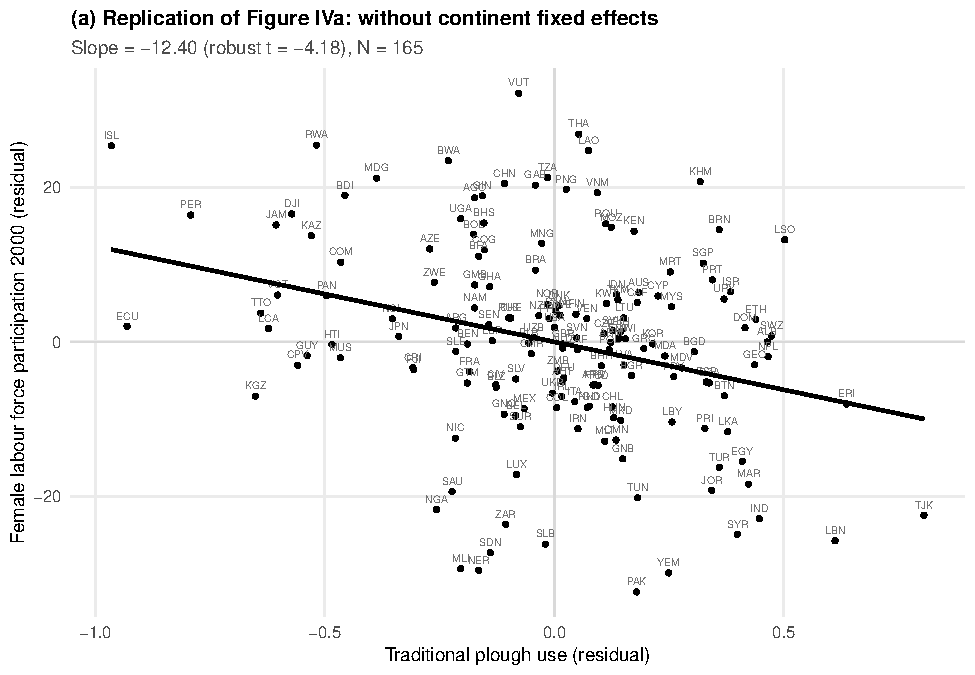
\includegraphics[width=\textwidth]{figures/figure_iva_replication.pdf}
\end{center}

\begin{center}
  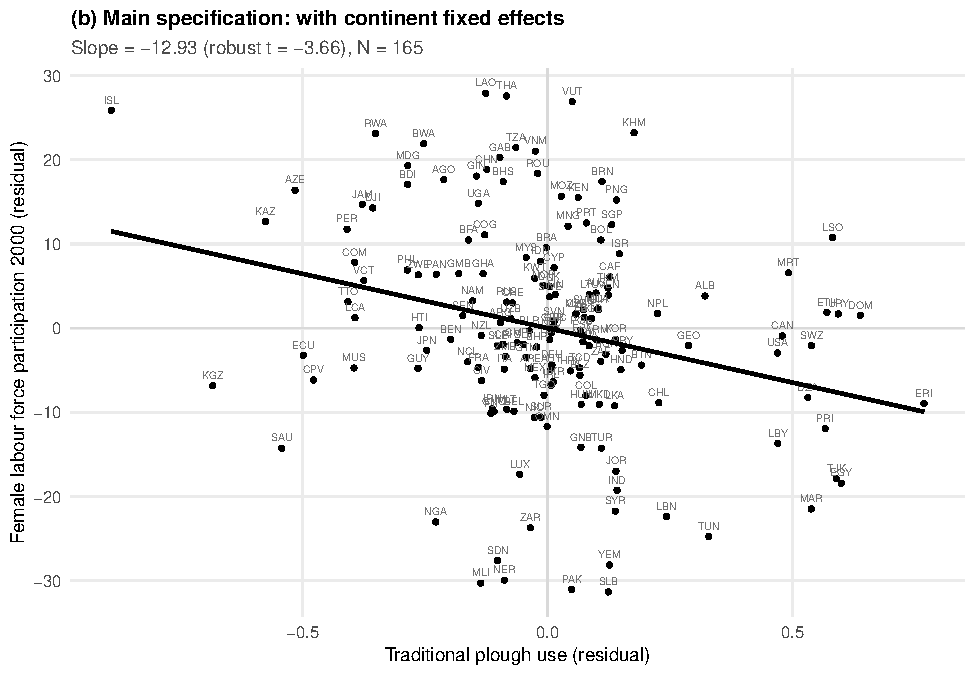
\includegraphics[width=\textwidth]{figures/figure_iva_continent_fe.pdf}
\end{center}

\subsection{Interpretation}

\instr{Appendix~B.2 shows how to read and interpret coefficients.}

A causal interpretation of $\beta$ requires that no omitted variable is correlated with both plough use and participation (mean-zero error assumption). As discussed in the methodology, two such biases are plausible. If societies that already had norms against women's work were more likely to adopt the plough, part of the effect of these norms would be attributed to the plough, making $\beta$ too negative. If, instead, more developed societies were more likely to adopt the plough and are today more open to women's work, $\beta$ would be pushed towards zero. We can examine the second argument for income. When we estimate our main specification without income on the same 165 countries, the coefficient changes from $-12.93$ to $-16.47$. The estimate thus becomes more negative when income is left out. This is surprising, because the methodology suggests the opposite. The U-shaped effect of income on participation explains this result (Goldin, 1995).

In poor countries, many women work out of necessity, for example in agriculture, and participation first falls as income rises before it increases again in rich countries. 72\% of our countries lie below the turning point of about USD 4'600, so for most of them a higher income goes along with fewer working women. At the same time, countries with a plough tradition have higher incomes today on average. Without income in the regression, part of the lower participation that is due to income is therefore attributed to the plough. The omitted variable bias is thus negative and makes $\beta$ too negative. This direction follows from the sign of the bias term $\delta \cdot b$. Here $\delta$ is the effect of income on participation from equation~\eqref{eq:ols}, and $b$ is the coefficient of plough use in a regression of income on plough use and the other controls. Since $b > 0$ and $\delta < 0$ for most countries, the bias $\delta \cdot b$ is negative. In our data it equals $-3.54$, which is exactly the difference between the two estimates. Since today's income cannot have caused plough adoption in the past, this correlation reflects either a common cause, such as historical development, or an effect of the plough on income. In the first case, the $-3.54$ is a bias and controlling for income is correct. In the second case, which is also mentioned in the methodology, income is a consequence of the plough. The plough would then lower participation partly through higher income, so this indirect path is part of the true plough effect. As we cannot tell the two cases apart, the total effect lies between $-12.93$ and $-16.47$.

What remains open is the first bias mentioned in the methodology, which is a form of reverse causality. Societies that already restricted women's work may have been more likely to adopt the plough. Such earlier norms are not observed and cannot be checked. To address these unobserved factors, the authors additionally use an IV strategy, which relies on instruments that are assumed to affect female labour force participation only through plough use.

We learn that plough ancestry is strongly associated with lower female labour force participation today, and our replication confirms the authors' numbers. Whether this association reflects a causal effect is examined with the IV estimates in the next section.

\subsection{IV results}

The replication of Table VIII, column (2), of Alesina, Giuliano and Nunn (2013) use a sample of 160 countries and includes historical controls, contemporary controls and continent fixed effects.

In the first stage (Panel A), the suitability of ancestral lands for crops for which the plough was more advantageous predicts traditional plough use more strongly than suitability for crops for which it was less advantageous. The coefficients are respectively 0.629 and 0.185 and the difference between them is statistically significant ($p=0.00267$). The joint F-statistic of 25.06 supports the relevance of the instruments.

In the reduced form (Panel B), the two measures of crop suitability are associated with female labour force participation in opposite directions. The coefficients are $-11.299$ and 19.571 and both are statistically significant at the 1\% level ($p=0.0093$ and $p=0.0024$).

The author's table assigns two stars to the coefficient of $-11.299$, indicating significance at 5\% level, even though the coefficient and its robust standard error of 4.285 match our replication after rounding.

In the second stage (Panel C), the 2SLS coefficient is $-25.01$, with a robust standard error of 7.513 ($p=0.0011$). Both values match the published results after approximation. Using the same sample, controls and fixed effects, the OLS coefficient is $-12.089$, with a robust standard error of 3.587. A 10 percentage point increase in the share of the population whose ancestors used the plough corresponds to a female labour force participation rate in 2000 that is about 1.2 percentage points lower according to the OLS estimate and about 2.5 percentage points lower according to the IV estimate.

The Hausman test ($p=0.0406$) rejects the null hypothesis that traditional plough use is exogenous at the 5\% level, conditional on instrument validity. The Hansen J test ($J=14.861$, $p=0.000116$) rejects the overidentifying restrictions. Under the estimated model, the data are therefore difficult to reconcile with the assumption that both instruments are uncorrelated with the error term. One possible explanation is that suitability for certain crops influenced female labour force participation through other channels, such as economic development. The test leaves open which instrument or channel accounts for the rejection. This result calls for caution in interpreting both the Hausman test and the IV estimate as evidence of a causal effect.

% ===========================================================================
\section{Critical Evaluation}
% ===========================================================================
\subsection{Threats to internal validity}

For $\beta$ to measure a causal effect, plough use must be uncorrelated with the error term, conditional on the controls: $E[\varepsilon_c \mid \text{Plough}_c, \mathbf{X}_c] = 0$. We discuss three reasons why this may fail and then ask whether the IV strategy solves them.

\paragraph{Threat 1: Pre-existing gender norms (OVB and reverse causality).}
As the authors themselves acknowledge, male-dominated societies may have been more likely to adopt the plough, so causality could also run from norms to plough use. If these norms were passed down, they also lower FLFP today and are part of the error term. Using the OVB formula,
\[
\text{bias} = \beta_z \cdot \frac{\operatorname{Cov}(\text{Plough}, z)}{\operatorname{Var}(\text{Plough})},
\]
plough use is positively correlated with unequal norms ($\operatorname{Cov} > 0$), and unequal norms reduce FLFP ($\beta_z < 0$). The bias is therefore negative, and OLS overstates the effect of the plough. Religion, one channel through which such norms are transmitted, gives a sense of the size: controlling for it reduces the coefficient from $-12.4$ to $-9.9$, about 20\% (Table VII, without continent fixed effects). Since religion is measured in 2000, it captures norms from before the plough only partly, so the true bias may be larger.

\paragraph{Threat 2: Development and income.}
Societies that adopted the plough were more developed, and their descendants are richer today. Because income is observed, we can measure this bias. When we drop log income and its square from our main specification, the coefficient moves from $-12.93$ to $-16.47$. Since two variables are omitted, the bias has two terms:
\[
\text{bias} = \delta_1 b_1 + \delta_2 b_2 = -33.98 + 30.44 = -3.54 ,
\]
where $\delta_1 = -32.69$ and $\delta_2 = 1.94$ are the coefficients on log income and its square in equation~\eqref{eq:ols}, and $b_1 = 1.04$ and $b_2 = 15.72$ are the coefficients on plough use in regressions of log income and its square on plough use and the other controls. The formula reproduces the gap exactly. The net sign is negative because of the U-shaped relationship between income and female participation (Goldin, 1995): 72\% of our countries lie below the turning point of about USD 4,600, where higher income goes along with fewer working women, and plough countries are richer on average. If income is partly a consequence of the plough, it is a bad control and part of the $-3.54$ belongs to the plough effect. The total effect would then lie between $-12.9$ and $-16.5$.

\paragraph{Threat 3: Measurement error.}
Each ethnic group is only coded as having used the plough or not, and these groups are then linked to today's countries through ancestry, so plough use is measured with error. Classical measurement error pulls the coefficient towards zero (attenuation bias), so OLS understates the effect. This works in the opposite direction to Threat 1.

\paragraph{Does the IV strategy solve these problems?}
The instruments are the suitability of ancestral land for crops that benefit strongly from the plough (wheat, barley, rye) and for crops that benefit little (sorghum, millet). Since gender norms cannot change soil or climate, the instruments can address the reverse causality in Threat 1, and 2SLS also corrects for classical measurement error. The 2SLS estimate ($-25.0$) is about twice as large in absolute value as OLS on the same 160 countries ($-12.1$), and the Hausman test rejects the exogeneity of plough use ($p = 0.04$). This contradicts Threat 1, which predicts that OLS is too negative, but is consistent with measurement error dominating.

However, the IV is only valid if crop suitability affects FLFP solely through plough use, i.e.\ $\operatorname{Cov}(Z, \varepsilon) = 0$. Because crop suitability reflects geography, regions suited to plough-positive and plough-negative crops may also differ in disease burden, economic development or the type of farm work the crops require. The authors control for overall agricultural suitability and tropical climate, but other differences may remain in the error term, and the data support this concern. The Hansen J test rejects ($J = 14.9$, $p < 0.001$), and suitability for plough-negative crops barely predicts plough use (first stage: $0.18$, $p = 0.17$) but strongly predicts FLFP (reduced form: $19.6$, $p = 0.002$). This points to a direct effect that does not run through the plough. Since Hansen J only tests whether the two instruments agree, it could not detect a case where both are invalid in the same way. Table~\ref{tab:threats} summarises the threats.

\begin{table}[htbp]
\centering
\caption{Threats to internal validity and their likely effect on the OLS estimate}
\label{tab:threats}
\small
\begin{tabular}{llll}
\hline
Threat & Direction of bias & Effect on $-12.9$ & Solved by IV? \\
\hline
Pre-existing norms & negative & overstated & only if exclusion restriction holds \\
Development and income & negative ($-3.5$) & controlled for & observed; possibly a bad control \\
Measurement error & towards zero & understated & yes, if error is classical \\
IV: exclusion restriction & unclear & -- & doubtful (Hansen J rejects) \\
\hline
\end{tabular}
\end{table}

\subsection{Overall assessment}

We find the paper's main claim convincing in direction but not in magnitude. The main threats bias the OLS estimate in opposite directions, and the IV strategy rests on a questionable exclusion restriction, so we cannot say whether $-12.9$ over- or understates the true effect. Still, the negative relationship holds across several outcomes, many additional controls (Table VII) and our own extension, and the evidence on children of immigrants, who live under the same institutions, makes a purely geographic or institutional explanation unlikely. We therefore consider it credible that traditional plough use contributed to today's gender norms, while the precise estimates should be interpreted with caution.

% ===========================================================================
\section{Extension and Robustness}
% ===========================================================================
 \subsection{Extension}

The baseline specification of Alesina, Giuliano and Nunn (2013) assumes that the relationship between historical plough use and contemporary gender outcomes is homogeneous across countries. However, if this relationship reflects the persistence of cultural norms, an important question is whether political institutions and economic development can weaken their transmission. We investigate two potential moderating factors. First, communist regimes actively promoted female employment through state policies and greater integration of women into the labour market. If institutional changes can counteract traditional gender norms, we expect the negative plough effect to be weaker in countries with a communist history. Second, economic development may reduce the importance of traditional gender roles through structural transformation, increased educational opportunities and changes in labour demand. We therefore expect the negative plough effect to decrease in magnitude as income rises.

\paragraph{Empirical strategy.}

We extend the OLS specification in Table IV of the original paper by introducing an interaction between historical plough use and a country-level moderator:
\begin{equation}
    Y_c = \alpha + \beta_1 \mathit{Plough}_c + \beta_2 Z_c
    + \beta_3 (\mathit{Plough}_c \times Z_c)
    + X_c'\gamma + \delta_r + \varepsilon_c.
    \label{eq:extension}
\end{equation}
The dependent variable, $Y_c$, represents female labour force participation (FLFP), female firm ownership or women's parliamentary representation. The moderator, $Z_c$, is either a dummy indicating communist history or centred log income per capita. We retain the historical and contemporary controls of the baseline specification, including the quadratic income term. In the income interaction specification, the linear income term is captured by $Z_c$.

Following our main replication specification, we include continent fixed effects, $\delta_r$, and use heteroskedasticity-robust standard errors. Specifications without continent fixed effects are reported as a robustness comparison.

The coefficient of interest is $\beta_3$. The marginal plough effect is given by: 
\begin{equation}
    \frac{\partial Y_c}{\partial \mathit{Plough}_c}
    = \beta_1 + \beta_3 Z_c.
    \label{eq:marginal_effect}
\end{equation}
For communist history, the estimated plough effect is $\beta_1$ in non-communist countries and $\beta_1+\beta_3$ in communist countries. For economic development, centring log income allows $\beta_1$ to be interpreted as the estimated plough effect at mean log income, using the mean of the available income data.

Under both hypotheses, we expect $\beta_3 > 0$, indicating an attenuation of the negative relationship between historical plough use and contemporary gender outcomes.

A causal interpretation requires conditional exogeneity of plough use, the moderator and their interaction. As discussed in the critical evaluation, this assumption may not hold.  Our estimates are therefore interpreted as conditional associations rather than causal effects.

\paragraph{Results: Communist history.}
Table~\ref{tab:ext_comm} presents the results for communist history. Across all specifications, the coefficient on traditional plough use remains negative and statistically
significant, indicating that the original paper's findings remain robust among non-communist countries.

Without continent fixed effects, the interaction coefficient for FLFP is positive but statistically insignificant ($1.239$, SE $=5.960$). When continent fixed effects are
included, the coefficient increases to $3.074$ (SE $=6.103$), but remains statistically insignificant. The interaction coefficients for female firm ownership ($-3.467$) and women's political representation ($-3.368$) are also statistically insignificant.

Moreover, Table~\ref{tab:ext_marginal} shows that the estimated marginal plough effect on FLFP in communist countries, $\beta_1+\beta_3$, remains negative, at approximately $-11.425$ percentage points in the specification with continent fixed effects, compared to $-12.933$ percentage points without fixed effects.

Overall, we find no statistically significant evidence that communist history weakens the relationship between historical plough use and contemporary gender outcomes. However, the large standard errors prevent us from ruling out economically meaningful differences between communist and non-communist countries.

\begin{table}[htbp]
\centering
\caption{Heterogeneity of the plough effect by communist history}
\label{tab:ext_comm}
\small
\setlength{\tabcolsep}{4pt}
\begin{tabular}{lcccccc}
\hline
 & \multicolumn{3}{c}{Without continent FE} & \multicolumn{3}{c}{With continent FE} \\
 & FLFP & Ownership & Politics & FLFP & Ownership & Politics \\
 & (1) & (2) & (3) & (4) & (5) & (6) \\
\hline
Traditional plough use      & $-14.173^{***}$ & $-16.033^{***}$ & $-4.914^{***}$ & $-14.499^{***}$ & $-15.599^{***}$ & $-4.390^{**}$ \\
                            & $(3.261)$ & $(4.167)$ & $(1.861)$ & $(4.043)$ & $(5.453)$ & $(2.126)$ \\
Communist history           & $5.555$ & $4.450$ & $3.493$ & $5.468$ & $3.570$ & $4.339^{*}$ \\
                            & $(4.739)$ & $(5.699)$ & $(2.607)$ & $(4.448)$ & $(5.858)$ & $(2.595)$ \\
Plough $\times$ Communist   & $1.239$ & $-0.221$ & $-1.592$ & $3.074$ & $-3.467$ & $-3.368$ \\
                            & $(5.960)$ & $(8.864)$ & $(3.839)$ & $(6.103)$ & $(9.650)$ & $(3.962)$ \\
\hline
Historical controls         & Yes & Yes & Yes & Yes & Yes & Yes \\
Income controls             & Yes & Yes & Yes & Yes & Yes & Yes \\
Continent fixed effects     & No  & No  & No  & Yes & Yes & Yes \\
Observations                & 164 & 122 & 143 & 164 & 122 & 143 \\
Adjusted $R^2$              & 0.385 & 0.105 & 0.271 & 0.383 & 0.115 & 0.276 \\
$R^2$                       & 0.422 & 0.179 & 0.322 & 0.439 & 0.225 & 0.352 \\
\hline
\end{tabular}

\tablenotes{OLS estimates of equation~\eqref{eq:extension} with $Z_c$ a
communist-history dummy. Heteroskedasticity-robust standard errors in
parentheses. * $p<0.10$, ** $p<0.05$, *** $p<0.01$.}
\end{table}

\begin{table}[htbp]
\centering
\caption{Marginal plough effect in communist countries ($\beta_1+\beta_3$)}
\label{tab:ext_marginal}
\small
\begin{tabular}{llcccc}
\hline
Outcome & Specification & Estimate & Robust SE & $p$-value & 95\% CI \\
\hline
FLFP                  & Without FE & $-12.933$ & $5.599$ & $0.021$ & $[-23.908,\ -1.959]$ \\
FLFP                  & With FE    & $-11.425$ & $5.636$ & $0.043$ & $[-22.471,\ -0.379]$ \\
Female firm ownership & Without FE & $-16.254$ & $8.617$ & $0.059$ & $[-33.144,\ 0.635]$ \\
Female firm ownership & With FE    & $-19.065$ & $9.114$ & $0.036$ & $[-36.928,\ -1.203]$ \\
Women in parliament   & Without FE & $-6.506$  & $3.758$ & $0.083$ & $[-13.873,\ 0.860]$ \\
Women in parliament   & With FE    & $-7.757$  & $3.938$ & $0.049$ & $[-15.475,\ -0.040]$ \\
\hline
\end{tabular}

\tablenotes{Sum of the plough and interaction coefficients from
Table~\ref{tab:ext_comm}. Confidence intervals use the normal approximation.}
\end{table}

\paragraph{Results: Economic development.}
Table~\ref{tab:ext_income} examines heterogeneity by economic development. At mean log income, the estimated plough coefficients remain negative and statistically significant
at the 1\% level across all three outcomes, both with and without continent fixed effects.

Contrary to our initial hypothesis, the interaction coefficients between historical plough use and log income are negative across all specifications. When continent fixed effects are included, the interaction coefficients for FLFP ($-2.592$, SE $=1.853$) and female firm ownership ($-1.198$, SE $=2.699$) remain statistically insignificant.

However, the interaction coefficient for women's political representation is negative and statistically significant at the 1\% level. Its magnitude increases from $-2.705$ without continent fixed effects to $-3.425$ (SE $=0.949$) when continent fixed effects are included.

This suggests that the negative relationship between historical plough use and women's political representation becomes stronger as income increases, rather than weaker as initially hypothesised. This finding is robust to the inclusion of continent fixed effects.

Overall, we find no evidence that economic development systematically attenuates the persistence of gender norms associated with historical plough use.

\begin{table}[htbp]
\centering
\caption{Heterogeneity of the plough effect by economic development}
\label{tab:ext_income}
\small
\setlength{\tabcolsep}{4pt}
\begin{tabular}{lcccccc}
\hline
 & \multicolumn{3}{c}{Without continent FE} & \multicolumn{3}{c}{With continent FE} \\
 & FLFP & Ownership & Politics & FLFP & Ownership & Politics \\
 & (1) & (2) & (3) & (4) & (5) & (6) \\
\hline
Traditional plough use      & $-12.952^{***}$ & $-16.206^{***}$ & $-5.505^{***}$ & $-13.716^{***}$ & $-17.469^{***}$ & $-6.306^{***}$ \\
                            & $(2.858)$ & $(4.213)$ & $(1.680)$ & $(3.440)$ & $(5.060)$ & $(1.876)$ \\
Log income (centred)        & $-2.599^{**}$ & $1.207$ & $3.153^{***}$ & $-1.761$ & $-0.842$ & $3.570^{***}$ \\
                            & $(1.208)$ & $(1.787)$ & $(0.685)$ & $(1.578)$ & $(2.168)$ & $(0.738)$ \\
Plough $\times$ Log income  & $-2.033$ & $-2.411$ & $-2.705^{***}$ & $-2.592$ & $-1.198$ & $-3.425^{***}$ \\
                            & $(1.619)$ & $(2.618)$ & $(0.981)$ & $(1.853)$ & $(2.699)$ & $(0.949)$ \\
\hline
Historical controls         & Yes & Yes & Yes & Yes & Yes & Yes \\
Income controls             & Yes & Yes & Yes & Yes & Yes & Yes \\
Continent fixed effects     & No  & No  & No  & Yes & Yes & Yes \\
Observations                & 165 & 123 & 144 & 165 & 123 & 144 \\
Adjusted $R^2$              & 0.369 & 0.105 & 0.298 & 0.362 & 0.122 & 0.316 \\
$R^2$                       & 0.404 & 0.171 & 0.343 & 0.416 & 0.222 & 0.383 \\
\hline
\end{tabular}

\tablenotes{OLS estimates of equation~\eqref{eq:extension} with $Z_c$ centred
log income per capita (income controls: centred log income and its square).
Heteroskedasticity-robust standard errors in parentheses.
* $p<0.10$, ** $p<0.05$, *** $p<0.01$.}
\end{table}

\paragraph{Interpretation and robustness.}

As discussed in the critical evaluation, the baseline OLS estimates may suffer from omitted variable bias and measurement error. Introducing interaction terms does not resolve these identification problems and may introduce additional sources of endogeneity.

Communist history is not randomly assigned and may capture other institutional, historical or geographical characteristics. Continent fixed effects account for broad regional differences but cannot eliminate all potential confounding factors. Similarly, contemporary income may itself be influenced by historical gender norms, making it a potentially endogenous moderator.

Furthermore, the imprecision of the interaction estimates limits our ability to identify heterogeneous relationships. Statistically insignificant coefficients should therefore not be interpreted as evidence that the plough effect is identical across countries.

Overall, the results provide limited evidence that political institutions or economic development weaken the persistence of gender norms associated with historical plough use.

\subsection{Ideal empirical strategy}

An ideal empirical strategy would exploit exogenous variation in political institutions while holding historical and cultural characteristics as constant as possible. One potential setting is the historical division of Germany into East and West Germany following the Second World War. While both regions shared a common national history, they were exposed to substantially different political and economic institutions for approximately four decades.

With unrestricted data availability, we would collect detailed regional information on historical plough use, pre-division gender norms, female labour force participation and socioeconomic characteristics, together with longitudinal data covering the periods before, during and after the division.

We could then implement a difference-in-differences design with a triple interaction between historical plough use, exposure to communist institutions and the post-division period:
\begin{equation}
\begin{aligned}
    Y_{it} = {} & \alpha_i + \lambda_t
    + \theta_1 (\mathit{East}_i \times \mathit{Post}_t) \\
    & + \theta_2 (\mathit{Plough}_i \times \mathit{Post}_t) \\
    & + \theta_3 (\mathit{Plough}_i \times \mathit{East}_i \times \mathit{Post}_t)
    + \varepsilon_{it}.
\end{aligned}
\label{eq:ideal_strategy}
\end{equation}
Here, $\alpha_i$ and $\lambda_t$ denote regional and time fixed effects, respectively. The coefficient $\theta_3$ captures whether exposure to communist institutions changed the relationship between historical plough use and female labour force participation relative to West Germany.

Identification would require parallel trends in the absence of the institutional change, including comparable trends across regions with different levels of historical plough use. Pre-treatment data would allow us to assess this assumption. Selective migration, pre-existing regional differences and other differential post-war shocks would also need to be addressed.

This approach would provide more credible evidence on whether political institutions can weaken the persistence of historical gender norms. Nevertheless, it would not automatically identify the causal effect of historical plough adoption itself.

For economic development, an analogous strategy would require exogenous variation in regional income that is independent of historical gender norms and does not directly affect gender outcomes through other channels. Such variation would help distinguish the moderating role of income from reverse causality and omitted variable bias.


% ===========================================================================
\section{Conclusion}
% ===========================================================================

% Your text

% ===========================================================================
\begin{thebibliography}{0}
% ===========================================================================
% Author-year style without numbers
\makeatletter\renewcommand\@biblabel[1]{}\makeatother
\setlength{\leftskip}{1.5em}\setlength{\itemindent}{-1.5em}

\bibitem{agn2013} Alesina, A., Giuliano, P., \& Nunn, N. (2013). On the origins of gender roles: Women and the plough. \textit{Quarterly Journal of Economics}, 128(2), 469--530.

\bibitem{boserup1970} Boserup, E. (1970). \textit{Woman's Role in Economic Development}. George Allen and Unwin.

\bibitem{goldin1995} Goldin, C. (1995). The U-shaped female labor force function in economic development and economic history. In T. P. Schultz (Ed.), \textit{Investment in Women's Human Capital and Economic Development} (pp.~61--90). University of Chicago Press.

\bibitem{pryor1985} Pryor, F. L. (1985). The invention of the plow. \textit{Comparative Studies in Society and History}, 27(4), 727--743.
\end{thebibliography}

% ===========================================================================
\clearpage
\appendix
\section{Replication Worksheets}
% ===========================================================================
\subsection{The paper at a glance}

{\renewcommand{\arraystretch}{1.4}%
\begin{tabularx}{\textwidth}{@{}>{\raggedright\arraybackslash}p{0.36\textwidth}L@{}}
\toprule
Field & Your entry \\
\midrule
Paper & Alesina, A., Giuliano, P.\ and Nunn, N.\ (2013), ``On the Origins of Gender Roles: Women and the Plough,'' \textit{Quarterly Journal of Economics}, 128(2), 469--530. DOI: 10.1093/qje/qjt005 \\
Replication package & \textbf{[TO DO: link to the replication package we used]} (files: \texttt{replicationcode\_AGN.do}, \texttt{crosscountry\_dataset.dta}, README) \\
Additional data sources & None \\
Outcome ($Y$) & Female labour force participation in 2000 (also: female firm ownership, women in parliament) \\
Treatment or variable of interest ($X$) & Traditional plough use: share of the population whose ancestors used the plough \\
Unit of observation & Country \\
Setting and period & Cross-section of up to 177 countries; outcomes measured around 2000; plough use from pre-industrial ethnographic data \\
Comparison & Countries whose ancestors used the plough vs.\ countries whose ancestors did not, conditional on historical and contemporary controls \\
Main method & OLS with continent fixed effects; IV-2SLS \\
Result replicated & Table III (cols.\ 1--2), Table IV (cols.\ 1--2), Table VIII (Panels A--C, col.\ 2), Figure IVa (scatter plot) \\
Software and version & R 4.6.2; packages \texttt{ivreg}, \texttt{sandwich} and \texttt{lmtest} \\
Code & \textbf{[TO DO: repository link]} \\
\bottomrule
\end{tabularx}}

\subsection{Key variables}

{\renewcommand{\arraystretch}{1.4}%
\begin{tabularx}{\textwidth}{@{}>{\raggedright\arraybackslash}p{0.25\textwidth}
  >{\raggedright\arraybackslash}p{0.25\textwidth}
>{\raggedright\arraybackslash}p{0.16\textwidth}
  L@{}}
\toprule
Role & Name in paper & Name in dataset & Definition and unit \\
\midrule
Outcome ($Y$) & Female labor force participation & \texttt{flfp2000} & Share of women in the labour force in 2000, in \% (range 12.6--90.5) \\
Variable of interest ($X$) & Traditional plough use & \texttt{plow} & Share of the population whose ancestors used the plough (Ethnographic Atlas v39, linked via Ethnologue, population-weighted); 0--1 \\
Instrument ($Z$), if IV & Plough-positive / plough-negative environment & \texttt{plow\_\allowbreak positive\_\allowbreak crops}, \texttt{plow\_\allowbreak negative\_\allowbreak crops} & Suitability of ancestral land for crops that benefit strongly (wheat, barley, rye) or little (sorghum, millet) from the plough (FAO-GAEZ); 0--1 \\
Main controls ($W$) & Historical: agricultural suitability, tropical climate, large animals, political hierarchies, economic complexity; contemporary: log income and its square; continent FE & \texttt{agricultural\_\allowbreak suitability}, \texttt{tropical\_\allowbreak climate}, \texttt{large\_\allowbreak animals}, \texttt{political\_\allowbreak hierarchies}, \texttt{economic\_\allowbreak complexity}, \texttt{ln\_\allowbreak income}, \texttt{ln\_\allowbreak income\_\allowbreak squared}, \texttt{continent} & Ancestry-weighted ethnographic and geographic measures; log real GDP per capita in 2000 \\
\bottomrule
\end{tabularx}}

\medskip\noindent
Sample: 165 observations (OLS, Table IV) and 160 observations (IV, Table VIII); 165 countries; 1 period (cross-section).

\subsection{Reconciling differences}

{\renewcommand{\arraystretch}{1.4}%
\begin{tabularx}{\textwidth}{@{}>{\raggedright\arraybackslash}p{0.45\textwidth}L>{\raggedright\arraybackslash}p{0.15\textwidth}@{}}
\toprule
Possible source & What we checked & Effect on $\beta$ \\
\midrule
Data version & Used the authors' original dataset from the replication package & None \\
Sample restrictions and missing values & Listwise deletion as in the original code; N matches (177 / 165 / 160) & None \\
Construction of variables (definitions, deflators, logs of zero) & Used the authors' constructed variables; no new variables created & None \\
Sample weights & No weights in original or replication & None \\
Fixed effects and dropped singletons & Continent dummies with Africa as base category, as in Stata & None \\
Standard errors (clustering, small-sample corrections) & OLS: HC1 (= Stata \texttt{, r}); IV: HC0 (= Stata \texttt{ivreg2, r}, no small-sample correction) & None; SEs match exactly \\
Software defaults (Stata, R, Python) & Original in Stata, replication in R; coefficients and SEs identical & None \\
Other (specify) & -- & -- \\
\bottomrule
\end{tabularx}}

\subsection{Threats to internal validity}

{\renewcommand{\arraystretch}{1.4}%
\begin{tabularx}{\textwidth}{@{}>{\raggedright\arraybackslash}p{0.18\textwidth}
  L
  >{\raggedright\arraybackslash}p{0.13\textwidth}
  L
  >{\raggedright\arraybackslash}p{0.14\textwidth}@{}}
\toprule
Threat & Potential mechanism in this paper & Direction of bias & Addressed by the authors & Convincing? \\
\midrule
Omitted variable(s) & Pre-existing gender norms (e.g.\ transmitted through religion) lower FLFP today and are correlated with plough use & Negative (OLS overstates) & Extra controls in Table VII (religion: $-12.4 \to -9.9$); IV & Partly: no control for pre-plough norms \\
Reverse causality & Male-dominated societies more likely to adopt the plough & Negative (OLS overstates) & IV with crop suitability (norms cannot change geography) & Partly: depends on exclusion restriction \\
Measurement error & Binary ethnographic coding; ancestry mapping to today's countries & Towards zero (OLS understates) & IV; could explain IV $>$ OLS & Yes, if error is classical \\
Sample selection & Countries with missing data dropped (177 $\to$ 165 $\to$ 160; smaller samples for ownership and politics) & Unclear & Robustness to different treatments of missing language data & Mostly \\
Other: invalid instruments & Crop suitability reflects geography, which may affect FLFP directly (disease, development, type of farm work) & Unclear & Controls for agricultural suitability and tropical climate & No: Hansen J rejects ($p < 0.001$); plough-negative crops predict FLFP but not plough use \\
\bottomrule
\end{tabularx}}

\subsection{Reproducibility checklist}

% Replace $\square$ by $\boxtimes$ (needs \usepackage{amssymb}) for each item you fulfil.
\begin{itemize}[label=$\square$, leftmargin=*, itemsep=2pt]
  \item A README file describes the folder structure, the software and package versions, and the order in which the scripts are run.
  \item One master script runs the whole analysis, starting from the raw data.
  \item The raw data are not modified; all cleaning is done in code.
  \item The code only uses relative file paths.
  \item Every table and figure in the report is produced by a script.
  \item Random seeds are set wherever results depend on simulation or bootstrapping.
\end{itemize}

\textit{Use of AI tools.} We used Claude (Anthropic) to discuss the paper's methods, to check our reasoning and numbers against the original replication files, and to help edit parts. All regressions were run by us in R, and we reviewed and verified all text and results in the report.

% ===========================================================================
\clearpage
\section{Notes on Methods}
% ===========================================================================

\instr{Delete this appendix before submitting.}

\subsection{Guide to evaluate identification methods}


\paragraph{Step 1: What is the model?}
Write the authors' main specification in one of the forms we used in class:
\begin{align*}
  \text{OLS:} \quad & y_i = x_i'\beta + \varepsilon_i = \beta_1 + \beta_2 x_{i2} + \dots + \beta_K x_{iK} + \varepsilon_i . \\
  \text{Panel data:} \quad & y_{it} = x_{it}'\beta + \alpha_i + d_t + \varepsilon_{it} \\
  \text{IV:} \quad & y_i = x_{1i}'\beta_1 + x_{2i}'\beta_2 + \varepsilon_i,
     \quad \text{with instruments } z_i' = [z_{1i}' \;\; x_{2i}']
\end{align*}
Which variable $x_{ik}$ is the variable of interest? Which variables are controls? If you use panel methods, what exactly is in $\alpha_i$ and $d_t$ in your paper? For IV, which variables are in $x_{1i}$ and which in $z_{1i}$?
 
\paragraph{Step 2: Which comparison identifies $\beta$?}
What do the authors compare to identify $\beta$. Is it a comparison across units, within the same unit over time, or between units that are affected differently by an instrument? Once $\alpha_i$ and $d_t$ are taken out, or once only the variation in $x_{1i}$ that comes from $z_{1i}$ is used, what variation is left?
 
\paragraph{Step 3: Which assumption allows a causal interpretation of $\hat{\beta}$?}
Think about the material covered in class. Which of the main assumptions have to be fulfilled to allow for a causal interpretation. For OLS we made five assumptions: linearity, mean-zero error, homoskedasticity, no serial correlation, and normal errors. Both panel data methods and IV make some additional assumptions or replace some of the assumptions with their own version. For panel data methods, we have seen that the estimators differ in what they assume about $Cov(x_{is}, \varepsilon_{it})$ and $Cov(x_{it}, \alpha_i)$. What does the estimator in your paper need? For IV, we discussed exogeneity and relevance. What do they imply and how do the authors make sure that they are fulfilled? 
 
\paragraph{Step 4: Is the assumption plausible?}
This should be the core of your evaluation of the paper. Some questions to guide you:
\begin{itemize}[leftmargin=*, itemsep=2pt]
  \item In general: We discussed three threats to the internal validity of OLS. Ask yourself: Could $y_i$ also affect the variable of interest? Is there a third variable that drives both? Is the variable of interest measured with error?
  \item In panel data: Which of these problems can fixed effects account for and which not? Could the outcome in one  period affect the explanatory variables in a later period?
  \item For IV: Why should the instrument move $x_{1i}$? Can you think of any channel through which it might affect $y_i$ directly, or be related to something in $\varepsilon_i$?
\end{itemize}
 
\paragraph{Step 5: What evidence do the authors provide?}
Which tests, robustness checks or figures do the authors use to support the assumption from Steps 3 and 4? For IV, what does the first stage show, and how large is the $F$-statistic? Does the evidence provided by the authors address the concerns you raised in Step~4, or does it test something else?
 
\paragraph{Step 6: How are standard errors computed?}
Recall what happens when (A3) or (A4) fails. Which standard errors do the authors report? Do they cluster? If so, at which level? Are the errors potentially correlated within these clusters?
 
\subsection{Interpreting coefficients}
 
\begin{tabularx}{\textwidth}{@{}P{0.3\textwidth}L@{}}
\toprule
\textbf{Specification} & \textbf{Interpretation of $\beta_k$} \\
\midrule
$y_i$ on $x_{ik}$ & A one-unit increase in $x_{ik}$ changes $y_i$ by $\beta_k$ units. \\
$\log y_i$ on $x_{ik}$ & A one-unit increase in $x_{ik}$ changes $y_i$ by about $100\beta_k$ percent (exactly $100(e^{\beta_k}-1)$ percent). \\
$y_i$ on $\log x_{ik}$ & A one percent increase in $x_{ik}$ changes $y_i$ by about $\beta_k/100$ units. \\
$\log y_i$ on $\log x_{ik}$ & A one percent increase in $x_{ik}$ changes $y_i$ by about $\beta_k$ percent (an elasticity). \\
Binary $y_i$ (linear probability model) & A one-unit increase in $x_{ik}$ changes the probability that $y_i = 1$ by $100\beta_k$ percentage points. \\
\bottomrule
\end{tabularx}
 
In each case, the other explanatory variables are held constant.

\subsection{Direction of omitted variable bias}

As in class, suppose the true model is $y_i = x_i'\beta + \gamma w_i + \varepsilon_i$, but you estimate $y_i = x_i'\beta + \varepsilon_i$ and omit $w_i$. Then
\[
  E(\hat\beta_k) = \beta_k + \gamma \, \hat\beta_{w\_on\_x,k} ,
\]
where $\gamma$ is the effect of $w_i$ on $y_i$ and $\hat\beta_{w\_on\_x,k}$ is the coefficient on $x_{ik}$ in a regression of $w_i$ on $x_i$. In panel data, $\alpha_i$ plays the role of $w_i$ when it is ignored.
 
\begin{center}
\begin{tabular}{@{}lcc@{}}
\toprule
 & \textbf{$w_i$ raises $y_i$ ($\gamma > 0$)} & \textbf{$w_i$ lowers $y_i$ ($\gamma < 0$)} \\
\midrule
$w_i$ positively correlated with $x_{ik}$ & Upward bias & Downward bias \\
$w_i$ negatively correlated with $x_{ik}$ & Downward bias & Upward bias \\
\bottomrule
\end{tabular}
\end{center}
 
Upward bias makes the estimate more positive. For a negative $\beta_k$, it therefore pulls the estimate toward zero, so always say whether the bias moves the estimate toward or away from zero.

\end{document}
